\subsection{GLM–HMM better explains choice data with dorsomedial striatum inhibition}
\label{sec:glmhmm:2.2.7}

The standard GLM describes choice as depending on a fixed linear combination of sensory evidence, trial history and the presence or absence of optical inhibition. However, an alternative possibility is that mice use a weighting function that varies over time. To test this idea, we adopted a latent state model with different GLM weights for different states (Fig. \ref{fig:glmhmm:4}). The model consists of a hidden Markov model (HMM) with Bernoulli GLM observations, or GLM–HMM \cite{bengio_input_1994,escola_hidden_2011,calhoun_unsupervised_2019,ashwood_mice_2022} (Fig. 5a,b). Each hidden state is associated with a unique set of GLM weights governing choice behavior in that state. Probabilistic transitions between states occur after every trial, governed by a fixed matrix of transition probabilities (\ref{sec:appendix1:methods}).

\begin{figure}[t!]
  \begin{center}
    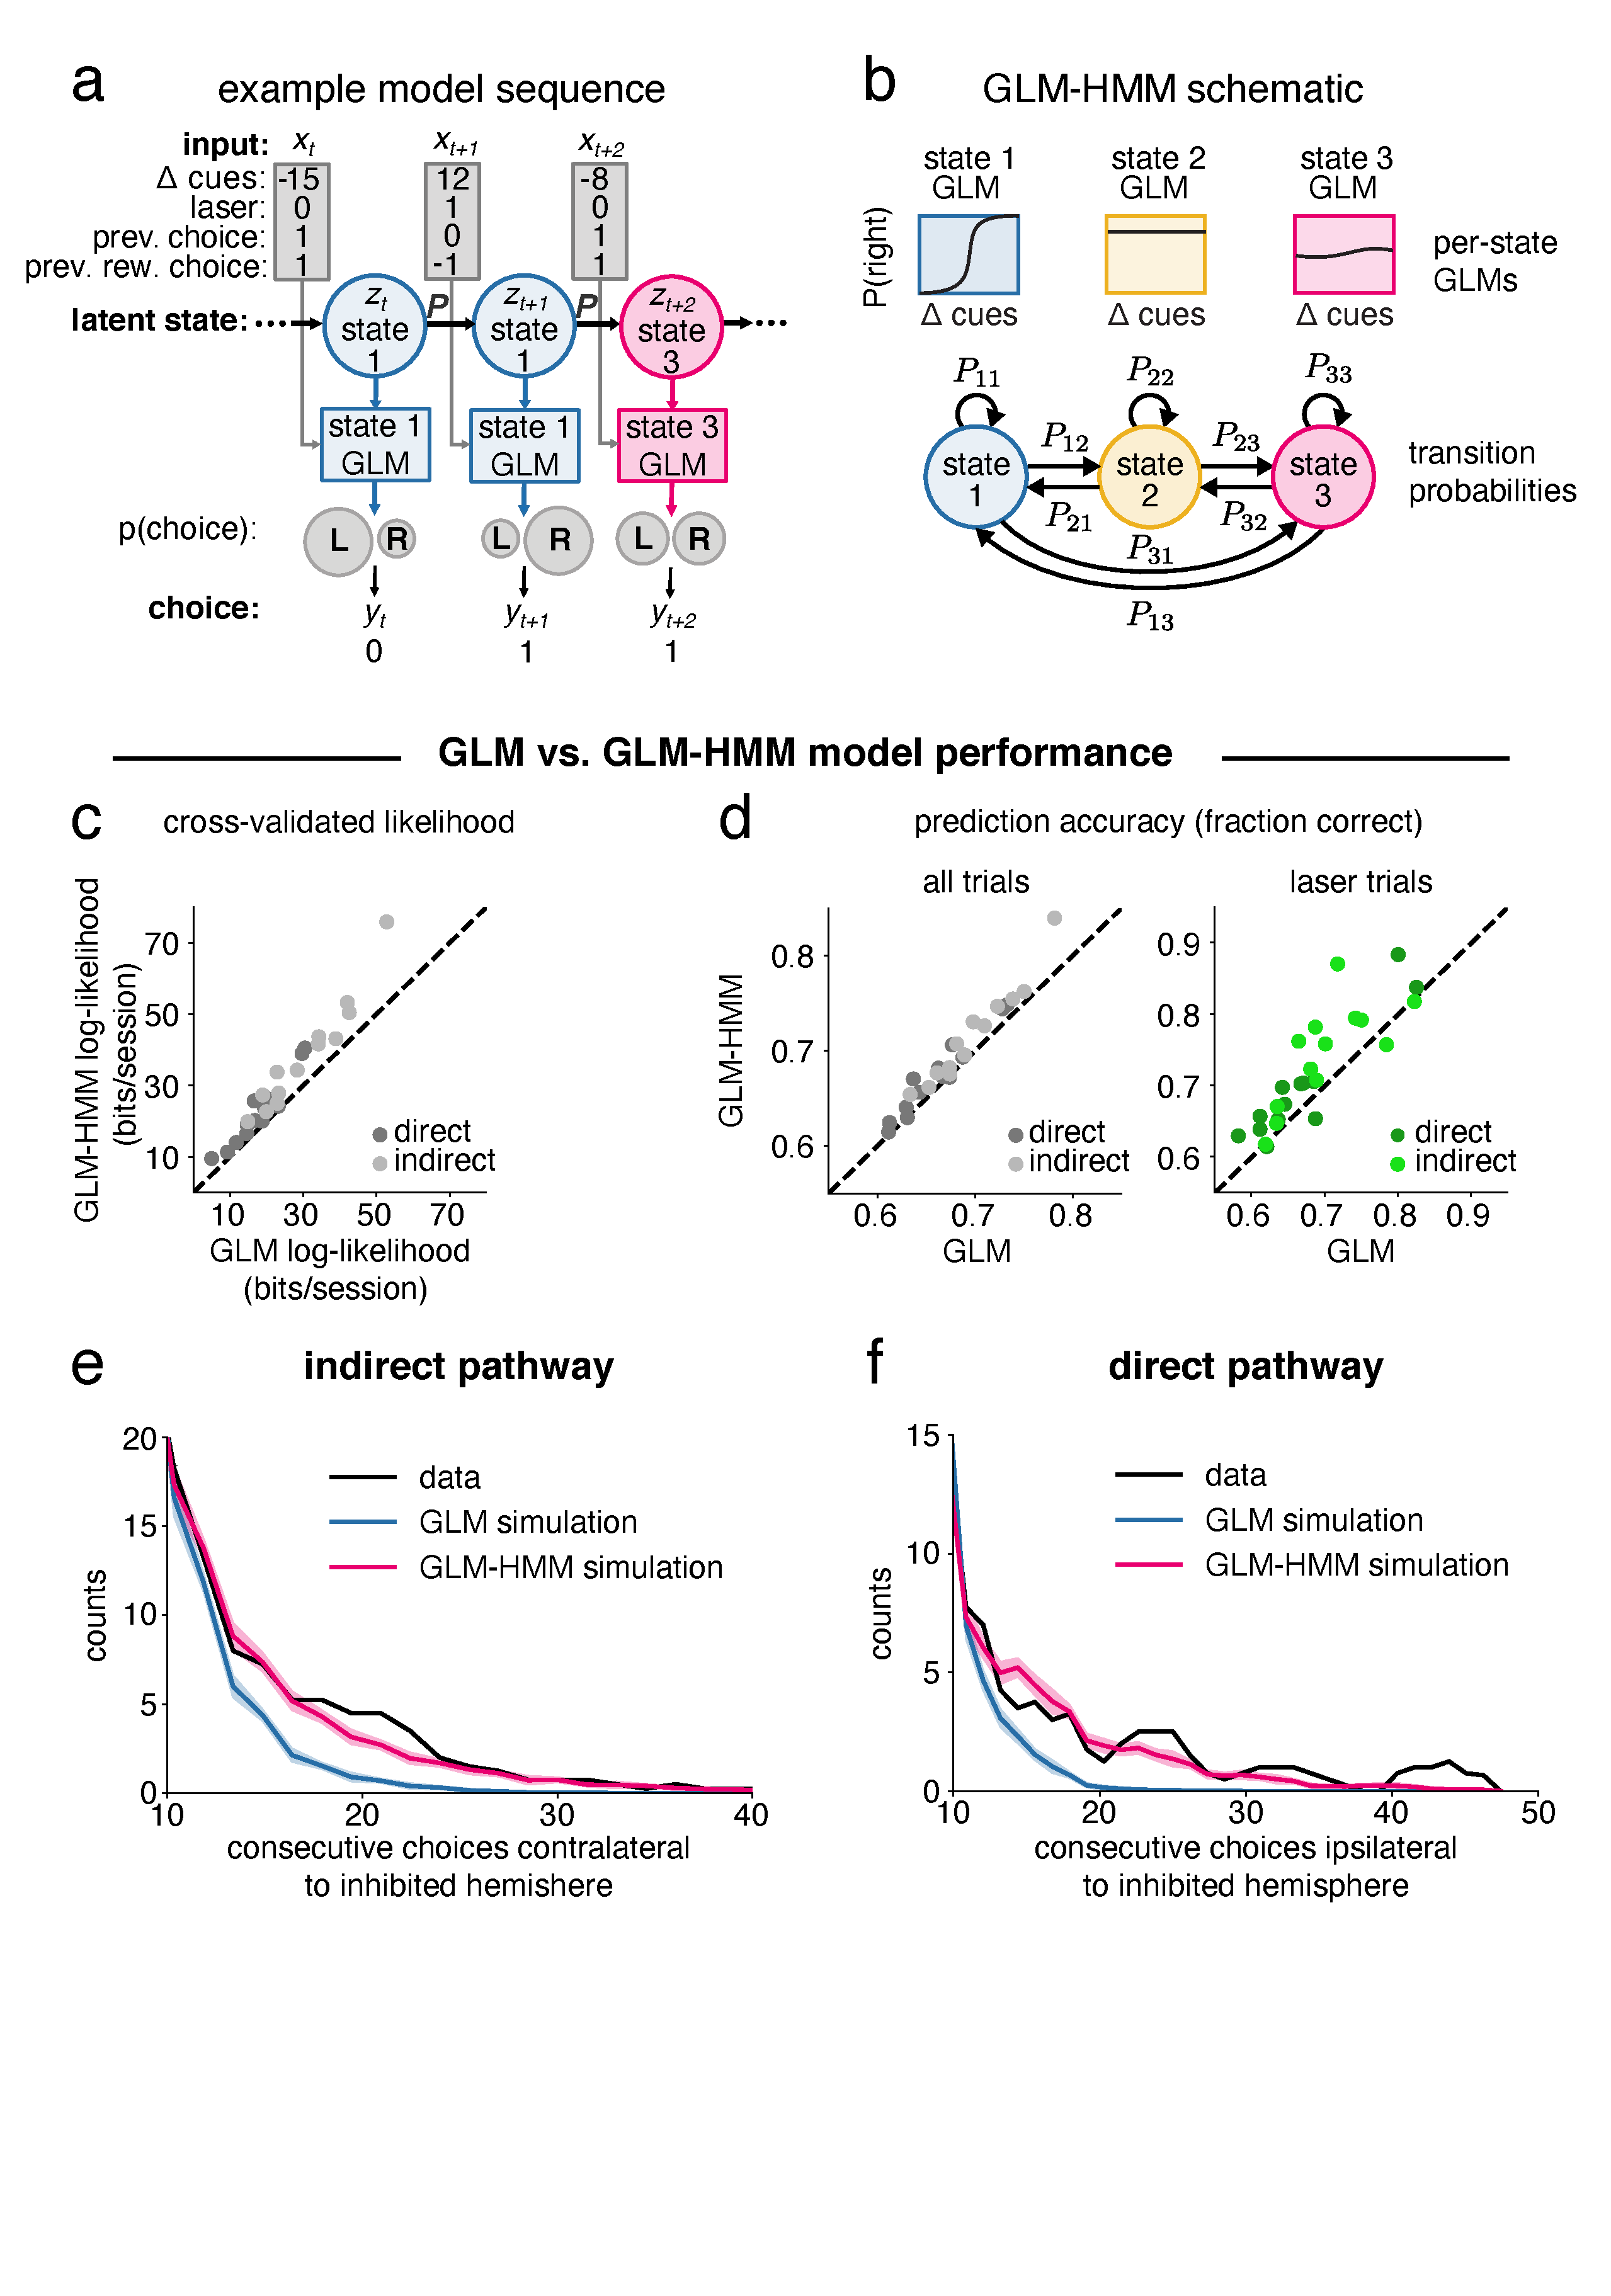
\includegraphics[width=0.90\linewidth]{ch2-glmhmm/glmhmm-figures/Fig5.pdf}
    \caption[A GLM–HMM better explains choice during the evidence accumulation task than the GLM, particularly on trials with dorsomedial striatum pathway inhibition]{\textbf{A GLM–HMM better explains choice during the evidence accumulation task than the GLM, particularly on trials with dorsomedial striatum pathway inhibition.} (a) Example sequence of 3 trials of the evidence accumulation task, showing the relationship between external covariates (inputs), latent state, and choice on each trial. On each trial, the latent state defines which GLM weights map inputs ($\Delta$ cues, laser, previous choice, and previous rewarded choice) to the probability of choosing right or left. The transition probability P governs the probability of changing states between trials. See \ref{sec:appendix1:methods} for information on how the inputs were coded. (b) Schematic of GLM-HMM. The model has 3 latent states with fixed probabilities of}
    \label{fig:glmhmm:5}
  \end{center}
  \vspace{-1.5cm}
\end{figure}
\begin{figure}[t!]
  \contcaption{transitioning between them. Each state is associated with a distinct decision-making strategy, defined by a mapping from external covariates, or inputs, such as $\Delta$ cues, to choice probability. (c) Cross-validated log-likelihood demonstrating the increased performance of the GLM-HMM over a standard Bernoulli GLM on held-out sessions. Dots represent model performance for individual mice (n=13 for each group). (d) Same as c but showing prediction accuracy as a fraction of the choices correctly predicted by each model across all trials (left) or on the subset of trials when the laser was on (right). (e) Histograms showing the number of consecutive laser trials for which the animal’s choice was in the same direction as the expected biasing effect of the laser (i.e. a choice contralateral to the laser hemisphere during DMS indirect pathway inhibition). Data (black), GLM simulation (blue), GLM-HMM simulation (pink). For the simulations, data of the same length as the real data was generated 100 times and the resulting histograms averaged. Curves denote smoothed counts using a sliding window average (window size = 3 bins). Shaded regions around the GLM and GLM-HMM curves indicate 95\% confidence intervals. (f) Same as e but for mice receiving direct pathway inhibition of the DMS, therefore laser-biased choices are defined as those ipsilateral to the hemisphere of inhibition.}% Continued caption
\end{figure}

The GLM–HMM explained the choice data in the evidence accumulation task better than the GLM across multiple measures. To compare models, we computed the test log-likelihood of each animal’s data using cross-validation with held-out sessions (three-state GLM–HMM in Fig. \ref{fig:glmhmm:5}; see Extended Data Fig. \ref{fig:ap1:ext7}a–e and \ref{sec:ap1:m10} for more information on model selection). The three-state GLM–HMM achieved an average of a 6.2 bits per session (bps) increase in log-likelihood, making an average session $\sim$76 times more likely under the GLM–HMM (Fig. \ref{fig:glmhmm:5}c). Furthermore, the GLM–HMM correctly predicted choice on held-out data more often than the GLM, especially on laser trials (Fig. \ref{fig:glmhmm:5}d; average improvement across mice of 1.6\% on all trials, 3.5\% on trials with optical inhibition and 4.1\% on trials with optical inhibition when considering only mice with at least 100 inhibition trials).

Most interestingly, the GLM–HMM was better able to capture the temporal structure in the effect of inhibition on choice. Specifically, the choice data contained long runs in which choice was consistent with the bias direction predicted by pathway-specific inhibition (‘laser’), a feature which GLM–HMM simulations recapitulated, but GLM simulations did not (Fig. \ref{fig:glmhmm:5}e,f). Thus, taken together, the GLM–HMM provided a better model of the choice data than a standard GLM, particularly on trials with pathway-specific DMS inhibition.